\documentclass[a4paper]{article}

% ---------- Encoding, lingua, font ----------
\usepackage[utf8]{inputenc}
\usepackage[T1]{fontenc}
\usepackage{textcomp}
\usepackage[italian]{babel}
\renewcommand{\familydefault}{\sfdefault}
\emergencystretch=1.5em
\usepackage{enumitem}   % nel preambolo

% ---------- Colori (UNA sola volta, prima di tikz/tcolorbox) ----------
\usepackage[dvipsnames,table]{xcolor}

% ---------- Matematica ----------
\usepackage{amsmath, amssymb, amsfonts, amsthm}
\usepackage{mathtools}
\DeclarePairedDelimiter\ceil{\lceil}{\rceil}
\DeclarePairedDelimiter\floor{\lfloor}{\rfloor}
\usepackage{cancel}
\usepackage{gensymb}

% ---------- Tabelle, figure, utilità ----------
\usepackage{booktabs, xltabular, tabularx, makecell}
\usepackage{subcaption}
\usepackage{float}
\usepackage{graphicx}
\usepackage{import}
\usepackage{pdfpages}
\usepackage{xifthen}
\pdfminorversion=7
\pdfsuppresswarningpagegroup=1
\graphicspath{{./figures/}}

\renewcommand{\arraystretch}{1.5}
\newcolumntype{Y}{>{\raggedright\arraybackslash}X}

% ---------- TikZ / pgfplots ----------
\usepackage{tikz}
\usetikzlibrary{shapes, arrows, automata, petri, decorations.markings,
                decorations.pathreplacing, positioning, calc, quotes}
\usepackage{circuitikz}
\usepackage{forest}
\usepackage{pgfplots}
\pgfplotsset{compat=1.18, width=10cm}

\tikzset{
    place/.style={circle, thick, draw=black, minimum size=6mm},
    state/.style={circle, thick, draw=black, fill=white, minimum size=6mm},
}

% ---------- Palette (solo quella nuova) ----------
\definecolor{thmcol}{HTML}{2563EB}   % blu     - teoremi
\definecolor{lemcol}{HTML}{7C3AED}   % viola   - lemmi
\definecolor{defcol}{HTML}{059669}   % verde   - definizioni
\definecolor{excol}{HTML}{EA580C}    % arancio - esempi
\definecolor{remcol}{HTML}{6B7280}   % grigio  - osservazioni

% ---------- Listings (riusa la palette nuova) ----------
\usepackage{listings}
\lstdefinestyle{mystyle}{
    backgroundcolor=\color{remcol!8},
    commentstyle=\color{defcol},
    keywordstyle=\color{thmcol},
    numberstyle=\tiny\color{remcol},
    stringstyle=\color{lemcol},
    basicstyle=\ttfamily\footnotesize,
    breakatwhitespace=false, breaklines=true, captionpos=b,
    keepspaces=true, numbers=left, numbersep=5pt,
    showspaces=false, showstringspaces=false, showtabs=false, tabsize=2
}
\lstdefinestyle{terminal}{
    backgroundcolor=\color{black},
    basicstyle=\ttfamily\color{green},
    frame=single, breaklines=true, showstringspaces=false
}
\lstset{style=mystyle}

% ---------- Teoremi, definizioni, esempi (tcolorbox) ----------
\usepackage[most]{tcolorbox}
\tcbuselibrary{theorems}

\tcbset{
  thmstyle/.style={
    enhanced, breakable, sharp corners,
    boxrule=0pt, frame hidden,
    borderline west={3pt}{0pt}{#1},
    colback=#1!6,
    colbacktitle=#1!14, coltitle=#1!60!black,
    fonttitle=\bfseries,
    titlerule=0pt,
    separator sign none,
    description delimiters parenthesis,
    before skip=12pt, after skip=12pt,
    left=8pt, right=8pt, top=4pt, bottom=4pt,
    overlay unbroken and first={\tikzset{external/export=false}},
    overlay middle and last={\tikzset{external/export=false}},
  }
}

\newtcbtheorem[number within=section]{theorem}{Teorema}{thmstyle=thmcol}{thm}
\newtcbtheorem[use counter from=theorem]{lemma}{Lemma}{thmstyle=lemcol}{lem}
\newtcbtheorem[use counter from=theorem]{definition}{Definizione}{thmstyle=defcol}{def}
\newtcbtheorem[use counter from=theorem]{example}{Esempio}{thmstyle=excol}{ex}
\newtcolorbox{remark}[1][]{thmstyle=remcol, title={Osservazione}, #1}

% ---------- Esercizi (mdframed) ----------
\usepackage{mdframed}
\theoremstyle{definition}
\newmdtheoremenv[
    linecolor=gray, leftmargin=0, rightmargin=0,
    innertopmargin=8pt, innerbottommargin=8pt
]{exercise}{Esercizio}[section]

% ---------- Figure svg ----------
\newcommand{\incfig}[1]{%
    \def\svgwidth{\columnwidth}
    \import{./figures/}{#1.pdf_tex}
}

% ---------- Hyperref (sempre per ultimo, prima di externalize) ----------
\usepackage{hyperref}
\hypersetup{colorlinks=false}

% ---------- Externalize ----------
\usetikzlibrary{external}
\tikzexternalize[prefix=figures/tikz/, optimize=false]
\tikzexternaldisable


\begin{document}
\begin{titlepage}
	\begin{center}
		\vspace*{1cm}

		\Huge
		\textbf{Machine Learning \& Deep Learning}

		\vspace{0.5cm}
		\LARGE
		UniVR - Dipartimento di Informatica

		\vspace{1.5cm}

		\textbf{Tommaso Toffali}

		\vfill


		\vspace{0.8cm}


		1° Semestre 2026/2027
    \end{center}
\end{titlepage}

\tableofcontents
\pagebreak
\part{Introduction to Machine Learning}
\section{What is Machine Learning?}
Machine Learning is a branch of Artificial Intelligence that enables
software to use data to find solutions to specific tasks without being explicitly
programmed to do so.
\subsection{Machine Learning vs Statistical Modelling}
In traditional statistical modelling, we follow a structured process:
\begin{enumerate}
    \item Collect data 
    \item Verify and clean the data (correct or discard if not clean)
    \item Use the clean data to test hypotheses, make predictions and forecasts
\end{enumerate}
In contrast, Machine Learning takes a different approach:
\begin{itemize}
    \item It is the \textbf{data} that determines which analytic techniques to use 
    \item The computer uses data to \textbf{train} algorithms to find patterns and make predictions 
    \item Algorithms are no longer \textbf{static} but become \textbf{dynamic}
\end{itemize}
\subsection{Conventional Programming vs Machine Learning}
The fundamental difference between conventional programming and machine learning can be undersood through their inputs and outputs:
\subsubsection{Conventional programming}
\begin{itemize}
    \item \textbf{Input}: Program + Data 
    \item \textbf{Output}: Result
    \item You write the program, give it data, and get results
\end{itemize}
\subsubsection{Machine Learning}
\begin{itemize}
    \item \textbf{Input}: Data + Result 
    \item \textbf{Output}: Result 
    \item You give the computer data and desired results, and it learns to generate a program/algorithm
\end{itemize}
\subsection{The Machine Learning Recipe}
\begin{definition}{Fundamental Steps of ML}
\centering Collect data \( \rightarrow \) Define models \( \rightarrow \) Define objective function \( \rightarrow \) Minimize error
\end{definition}
The ML recipe consists of 4 fundamental step:
\begin{enumerate}
    \item Collect data 
    \item Define a family of possible models
    \item Define an objective (error) function to quantify how well a model fits the data 
    \item Find the model that minimize the error function (training/learning a model)
\end{enumerate}
\subsubsection{The Key ingredients}
\begin{example}{Essential Ingredient}
\centering    Task \( \bullet \) Data \( \bullet \) Model \( \bullet \) Objective Function \( \bullet \) Learning Algorithm 
\end{example}
Every machine learning problem requires five essential ingredients:
\begin{itemize}
    \item \textbf{Task}: The problem we want to solve 
    \item \textbf{Data}: The information we use to learn 
    \item \textbf{Model hypothesis}: The family of functions we consider 
    \item \textbf{Objective function}: How we measure success 
    \item \textbf{Learning algorithm}: How we fine the best model
\end{itemize}
\section{Machine Learning Tasks}
A task represent the type of prediction being made to solve a problem on some data. We can 
identify a task with the set of functions that can potentially solve the problem. In generale, it 
consists of functions assigning each \textbf{input} \( x \in \mathcal{X} \) an \textbf{output} \( y \in \mathcal{Y} \).
\subsection{Classification task}
\begin{definition}{Classification}
\centering    Find a function \( f \in \mathcal{Y}^{\mathcal{X}} \) assigning each input 
    \( x \in \mathcal{X} \) a \textbf{discrete} label, \( f(x) \in \mathcal{Y} = \left\{ c_1, \ldots, c_k \right\} \).
\end{definition}
In classification, the output space is a finite set of discrete categories or classes. The goal is to learn 
a decision boundary that separates different classes.
\subsection{Regression task}
\begin{definition}{Regression}
\centering    Find a function \( f \in \mathcal{Y}^{\mathcal{X}} \) assigning each input 
    \( x \in \mathcal{X} \) a \textbf{continuos} label, \( f(x) \in \mathcal{Y} = \mathbb{R} \).
\end{definition}
In regression, the output is a continuos value, allowing for predictions of quantities such as prices, temperatures, or probabilities.
\subsection{Density Estimation task}
\begin{definition}{Density Estimation}
\centering Find a probability distribuition \( f \in \Delta(\mathcal{X}) \) that best 
fits the data \( x \in \mathcal{X} \).
\end{definition}
There is no reference to an output space (as in calssification and regression task). Instead, we 
make a reasoning on the \textbf{input} \( x \) itself, trying to model the underlying probability 
distribution that generated the data.
\subsection{Clustering task}
\begin{definition}{Clustering}
\centering Find a function \( f \in \mathbb{N}^{\mathcal{X}} \) that assigns each input
\( x \in \mathcal{X} \) a \textbf{cluster index} \( f(x) \in \mathbb{N} \). 
\end{definition}
All points mapped to the same index form a cluster. The goal is to group similar data points 
together without prior knowledge of the groups.
\subsection{Dimensionality Reduction Task}
\begin{definition}{Dimensionality Reduction}
\centering Find a function \( f \in \mathcal{Y}^{\mathcal{X}} \) that \textbf{maps} each (\textbf{high-dimensional}) 
input \( x \in \mathcal{X} \) to a \textbf{lower-dimensional} embedding \( f(x) \in \mathcal{Y} \), where \( dim(\mathcal{Y}) < dim(\mathcal{X}) \). 
\end{definition}
\section{Data in Machine Learning}
\subsection{Data representation}
We represent inputs of out algorithm as \( x \in \mathcal{X} \) and output as \( y \in \mathcal{Y} \). The dataset is the set of both,
where each input is associated with an output.
\vspace{1em}
\noindent
\newline
\textbf{Key consideration}:
\begin{itemize}
    \item The quality of the data is crucial for the performance of the algorithm 
    \item It is equally important to have a large amount of data to learn effective models
    \item Poor quality or insufficient data can lead to poor model performance 
\end{itemize}
\subsection{Features}
\begin{definition}{Features}
\centering Features are the measurable properties or charateristics of the phenomenon being observed
\vspace{1em}
\noindent
\newline
\textbf{Examples}:
\begin{itemize}
    \item To identify a flower: color, petal length, petal width, sepal length, sepal width 
    \item To identify a fruit: color, shape, size, texture, weight 
    \item To classify images: pixel values, edges, textures, shapes 
\end{itemize}
We can say that features are how algorithm "sees" the data and are in general represented 
with (fixed-size) vectors.
\end{definition}

\section{Data Distributions and Learning Types}
In machine learning, the information about the problem we want to solve
is represented in the form of a data distribution, usually denoted as \( p_{data} \).
\subsection{Supervised learning}
\subsubsection{Classification and Regression}
The data distribution is over pairs of inputs and outputs:
\[
  p_{data} \in \Delta(\mathcal{X} \times \mathcal{Y})
\]
Here:
\begin{itemize}
    \item \( \mathcal{X} \) is the input space 
    \item \( \mathcal{Y} \) is the output space (labels or targets)
    \item The goal is to learn a mapping from inputs to outputs using labeled data
\end{itemize}
\subsection{Unsupervised Learning}
\subsubsection{Density Estimation, Clustering and Dimensionality reduction}
The data distribution is only over the input space:
\[
  p_{data} \in \Delta(\mathcal{X})
\]
Here:
\begin{itemize}
    \item We do not have explicit labels or targets 
    \item The goal is to discover structure, patterns or representations within the data itself
\end{itemize}
\subsection{Summary of Learning Types}
\begin{center}
    \begin{tabular}{ |c|c|c| }
        \hline 
        \textbf{Task type} & \textbf{Data distribution} & \textbf{Learning Type} \\
        \hline 
        Classification, Regression & \( p_{data} \in \Delta(\mathcal{X} \times \mathcal{Y}) \) & Supervised Learning \\
        \hline
        Density Estimation, Clustering, Dimensionality Reduction & \( p_{data} \in \Delta(\mathcal{X}) \) & Unsupervised Learning \\
        \hline
    \end{tabular}
\end{center}
\textit{Note}. In \textbf{supervised learning}, each data point consistes of an input and corresponding 
output (label). In \textbf{unsupervised learning}, each data point consists only of the input, and the algorithm 
tries to find pattersn or structure without explicit labels.
\vspace{1em}
\noindent
\newline
The distinction is fundamental in machine learning, as it determines the type of 
algorithms and approaches used to solve different problems.
\section{Data sampling and dataset splitting}
\subsection{The data distribution problem}
In both supervised and unsupervised learning, the true data distribution \( p_{data} \) is typically \textbf{unknown}. This presents a fundamental 
challenge:
\begin{itemize}
    \item We do not have direct access to the underlying probability distribution that generates data 
    \item We only have access to a finite sample of data points drawn from this distribution
\end{itemize}
\textbf{Solution}: We perform \textbf{sampling} from the distribution. By collecting a representative sample of data, we can approximate the true 
distribution and use it to train our models.
\subsection{Training, Validation and Test sets}
To properly evaluate machine learning models, we split out data into three distinct sets. Each set serves a specific purpose 
inthe machine learning pipeline.
\begin{definition}{Dataset Splitting}
\centering 
A dataset is typically divided into three subsets:
\begin{itemize}
    \item \textbf{Training set} (\( D_{train} \)): Used to train the model 
    \item \textbf{Validation set} (\( D_{val} \)): Used to tune hyperparameters and select the best model 
    \item \textbf{Test set} \( (D_{test}) \): Used to evaluate the final model performance
\end{itemize}
\end{definition}
\begin{definition}{Critical Requirement}
\centering 
All three sets (training, validation, test) must be sampled from the \textbf{same probaility distribution}
\end{definition}
\subsection{How to use the three sets}
The three datasets serve different purposes in the machine learning workflow:
\subsubsection{Learning/Training Phase}
During the learning pahse, the \textbf{training set} is used to train the machine learning algorithm, which learns patterns and realtionships 
in the data to produce a \textbf{program} (model)
\vspace{1em}
\noindent
\newline
The \textbf{validation set} plays a crucial role in this phase:
\begin{itemize}
    \item Evaluates different model configurations 
    \item Tunes hyperparameters 
    \item Selects the best performing model
\end{itemize}
This process involves iterative feedback between training and validation until we find the optimal configuration.
\subsubsection{Testing/Model evaluation Phase}
Once the best model is selected, we use the \textbf{test set} to evaluate its performance. The trained model is applied 
to the test data, which it has never seen before. This gives us an unbiased estimated of how well the model will perform in real-world scenarios,
telling us whether out model can truly generalize to new data.
\subsection{The importance of Distribution similarity}
\subsubsection{Correct Scenario: Same Distribution}
When training, validation, and test sets are sampled from the \textbf{same distribution}:
\begin{itemize}
    \item The sets are \textbf{similar} in terms of statistical properties 
    \item They represents the same underlying phenomenon 
    \item However, they \textbf{do not overlap} (no data point appears in multiple sets)
\end{itemize}
This ensures that the model cna generalize well from training to test data.
\begin{example}{Fruits}
\centering
If we're classifying fruits, all three sets might contain apples and bananas in similar proportions, but with different specific instances.
\end{example}
\subsubsection{Incorrect Scenario: Different Distribution}
When training/validation and test come from \textbf{different distributions}, the model learns patterns from one distribution but is tested on another.
This problematic scenario typically leads to:
\begin{itemize}
    \item Poor performance on the test set 
    \item Unrealiable predictions on new data 
    \item Inability to generalize to real-world applications
\end{itemize}
\begin{example}{Different distributions}
\centering
Training on apples and bananas, but testing on oranges and limes. The model cannot calssify fruits it has never seen during training
\end{example}
\begin{theorem}{Key principle}
\centering
Training and test data must come from the \textbf{same distribution}, violating thi leads to poor generalization
\end{theorem}
    
\section{Training and Testing: The role of features}
\subsection{Training (Learning, Induction)}
During the training phase, the model learns to distinguish between different classes based on the features provided in the training 
data.
\begin{example}{Fruit classification}
\centering 
Consider a fruit classification task with the following training data:
\begin{itemize}
    \item \textit{red, round, leaf, 3oz, \( \ldots \)} \( \rightarrow \) apple 
    \item \textit{green, round, no leaf, 4oz, \( \ldots \)} \( \rightarrow \) apple 
    \item \textit{yellow, curved, no leaf, 8oz, \( \ldots \)} \( \rightarrow \) banana 
    \item \textit{green, curved, no leaf, 7oz, \( \ldots \)} \( \rightarrow \) banana
\end{itemize}
The model learns to associate patterns in the features (color, shape, presence of leaf, weight) with the corresponding labels (apple or banana).
\textbf{What distinguishes apples and bananas is based on the features!} The model identifies which feature combinations 
are characteristic of each class.
\end{example}
\subsection{Testing}
Once trained, the model can classify new examples based on the same features it learned during training.
When presented with a new example described byt the same semantic features, the model make a prediction 
\begin{example}{Fruit}
\centering 
Given a new fruit with features \textit{red, round, no leaf, 4oz, \( \ldots \)}, the model uses the 
learned patterns to predict whether it is an apple or banana.
\end{example}
\begin{theorem}{Critical Assumption}
\centering 
THe features of training and testing data \textbf{must be the same!}. The model can only make 
predictions based on features it was trained on
\end{theorem}
\subsection{Learning and Generalization}
Learning is fundamentally about \textbf{generalizing} from the training data. The goal is not simply to memorize the training examples,
but to learn patterns that apply to new, unseen data.
\vspace{1em}
\noindent 
\newline
However, the failure of a machine learning algorithm is foten caused by a \textbf{bad selection of training samples}.
The key issue is that we might introduce \textbf{unwanted correlations} from which the algorithm derives \textbf{wrong conclusions}.
\begin{example}{Recognize object in images}
\centering 
Consider a model trained to recognize objects in images. If all training images were captured on sunny days, the model might 
learn to associate sunny weather conditions with the objects. When tested on images taken on cloudy days, the model might
fail to recognize the same objects because it never encountered cloudy cnditions during training. The model incorrectly 
learned that sunny weather is a relevant feature for object recognition.
\vspace{1em}
\noindent
\newline
\textit{Quality and diversity of training data are crucial}. Training data should be representative of all real-world 
conditions
\end{example}
\section{The complete Machine Learning Recipe}
We can now revisit the complete machine learning workflow with all its essential ingredients:
\subsection{The five ingredients of Machine Learning}
Every machine learning problem requires five fundamental components that work toghether:
\begin{enumerate}
    \item \textbf{Task}: The specific problem we want to solve (e.g., classify birds vs. non-birds in images)
    \item \textbf{Data}: The collection of examples used to train and evaluate the model. Data quality and quantity are critical for success
    \item \textbf{Model Hypothesis}: The family of function or models we consider as a potential solutions. 
        This defines the space of possible models the learning algorithm can explore.
    \item \textbf{Objective Function}: A mathematical function that quantifies how well a model performs on the data. The learning algorithm aims to optimize this function 
    \item \textbf{Learning Algorithm}: The method used to search through the model hypothesis space and find the model that optimizes the objective function.
\end{enumerate}
\subsection{The interplay of Ingredients}
These five ingredients are interconnected:
\begin{itemize}
    \item The \textbf{task} determines what kind of \textbf{data} we need and what \textbf{model hypothesis} is appropriate 
    \item The \textbf{data} influences which features are available and how we define the \textbf{objective function} 
    \item The \textbf{model hypothesis} constrains what the \textbf{learning algorithm} can discover 
    \item The \textbf{objective function} guides the \textbf{learning algorithm} toward better models
\end{itemize}
Understanding and carefully selecting each ingredient is essential for building effective machine learning systems.
\section{Model and Hypothesis Space}
\subsection{What is a Model?}
\begin{definition}{Model}
\centering 
A \textbf{model} is the implementation of a function \( f \in \mathcal{F}_{\text{task}} \) that can be 
tractably computed.
\end{definition}
IN practice, when searching for our function \( f \), we don't look at everything in \( \mathcal{F}_{\text{task}} \). Instead, 
we look at a subset called the \textbf{hypothesis space}: \( \mathcal{H} \subset \mathcal{F}_{\text{task}} \), which is composed of a set of models 
(e.g., neural networks, decision trees, linear models).
\vspace{1em}
\noindent
\newline
The learning algorithm seeks a \textbf{solution within the hypothesis space}. In other words, a model is a simplified 
representation of the world that we can actually compute and optimize.
\vspace{1em}
\noindent
\newline
\textit{Observation}. The choice of hypothesis space is crucial:
\begin{itemize}
    \item If \( \mathcal{H} \) is too small, it may not contain a good solution 
    \item If \( \mathcal{H} \) is too large, finding the best model becomes computationally intractable 
    \item The hypothesis space defines the types of patterns the model can learn
\end{itemize}
\subsection{Types of Learning Paradigms}
\begin{definition}{Three Learning Paradigms}
\centering 
Machine learning can be categorized into different paradigms based on the type and availability of labeled data:
\vspace{1em}
\noindent
\newline
\textbf{Supervised learning}
\vspace{1em}
\noindent
\newline
In supervised learning, we have labeled data where each input is paired with its corresponding output. This includes:
\begin{itemize}
    \item \textbf{Classification}: Predicting discrete labels 
    \item \textbf{Regression}: Predicting continuous values 
\end{itemize}
\vspace{1em}
\noindent
\newline
\textbf{Unsupervised learning}
\vspace{1em}
\noindent
\newline
In unsupervised learning, we only have input data without labels. The goal is to discover 
structure in the data. That includes:
\begin{itemize}
    \item \textbf{Clustering}: Grouping similar data points 
    \item \textbf{Density estimation}: Modeling the probability distribution of data
    \item \textbf{Dimensionality Reduction}: Finding lower-dimensional representations
\end{itemize}
\end{definition}
\subsubsection{Supervised Learning}
In supervised learning, we have labeled data where each input is paried with its corresponding output.
\subsubsection{Unsupervised Learning}
In unsupervised learning, we only have input data without labels.
\subsubsection{Semi-Supervised Learning}
Semi-supervised learning addresses scenarios where we have a large amout of unlabeled data and only some
labeled examples. This paradigm has gained significant popularity in recent years
to leverage large dataset through self-supervised learning techniques.
\vspace{1em}
\noindent
\newline
The key idea is to provide the model with tasks different from the one to be solved, but that allow 
the model to learn the data distribution from the unlabeled data. Once the model understands the general structure of 
the data, it can then specialize on the few labeled examples to solve the target task.
\begin{example}{Training a language}
\centering 
Training a language model on large amounts of unlabeled text to learn general 
laguage pattern, then fine-tuning it on a small labeled dataset for sentiment analysis.
\end{example}
\section{Model-Based vs. Instance-Based Learning}
Machine learning algorithms can be further categorized based on how they make predictions:
\subsection{Model-Based (Parametric Learning)}
\begin{definition}{Parametric Model}
\centering 
A learning model that summarizes data with a \textbf{set of parameters of fixed size} (independent of the number 
of training examples) is called \textbf{parametric model}.
\vspace{1em}
\noindent
\newline
\textbf{Parametric Model Characteristics}
\vspace{1em}
\noindent
\newline
Key characteristics:
\begin{itemize}
    \item The model learns a fixed set of parameters from the training data 
    \item Once trained, the original training data can be discarded 
    \item No matter how much data you give to a parametric model, it won't change its mind about how many parameters it needs.
    \item The model makes predictions using only the learned parameters
\end{itemize}
\textbf{Examples}: Naive Bayes, Linear regression, Logistic Regression, Neural Networks.
\end{definition}
In a model-based approach, the algorithm learns a function (e.g., decision boundary) described by parameters. For instance, a linear classifier might 
learn the curve \( \alpha x_1 + \beta x_2 + \gamma \) that separates 
two classes, where \( \alpha, \beta, \gamma \) are the parameters.
\subsection{Instance-Based (Nonparametric) Learning}
\begin{definition}{Nonparametric Model}
\centering 
These algorithms \textbf{do not learn parameters} but instead use the data itself to compare a new example 
through similarity metrics.
\vspace{1em}
\noindent
\newline
\textbf{Nonparametric Model characteristics} 
\vspace{1em}
\noindent
\newline
Key characteristics:
\begin{itemize}
    \item The models stores (some or all of) the training data
    \item Predictions are made by comparing new examples to stored training examples 
    \item The model's complexity can grow with the amount of training data
    \item No explicit training phase that produces a fixed set of parameters
\end{itemize}
\textbf{Example}: K-Nearest Neighbors (KNN), Support Vector Machines (SVM), Random Forest.
\end{definition}
In an instance-based approach, when a new example arrives, it is compared with nearby training 
examples and classified according to a similarity policy. For example, in KNN, a new point is 
classified based on the majority class of its \( k \) nearest neighbors in the training data.
\section{Error Function (Objective Function)}
To allow an algorithm to learn, we need to provide it with a metric, a measure that helps it understand the direction of the optimal solution we are 
seeking. For this reason, \textbf{performance measures} are defined to enable the algorithm to learn.
\begin{center}
    \begin{tabular}{ |c|c|c| }
        \hline 
        \textbf{Aspect} & \textbf{Model-based} & \textbf{Instance-Based} \\
        \hline 
        Parameters & Fixed number of parameters & No fixed parameters \\
        \hline 
        Training data & Can be discarded after training & Must be retained for predictions \\
        \hline
        Prediction speed & Fast (onlu uses parameters) & Slower (compares with stored data) \\
        \hline 
        Memory & Low (stores only parameters) & High (stores training examples) \\
        \hline 
        Flexibility & Fixed model complexity & Complexity grows with data \\
        \hline
    \end{tabular}
\end{center}
\subsection{What is an Error function?}
In machine learning, \textbf{training a model} means finding a \textbf{function} which maps a set of values \( x \) to 
a value \( y \). we can calculate how well a predictive model is doing by comparing the \textbf{predicted values} with the \textbf{true values}
for \( y \).
\begin{definition}{Training error vs. Test Error}
\centering 
\begin{itemize}
    \item If we apply the model to the data it was trained on, we are calculating the \textbf{training error}
    \item If we calculate the error on data which was \textbf{unknown} in the training phase, we are calculating the \textbf{test error}
\end{itemize}
The test error is the most important metric because it tells us how well the model generalizes 
to new, unseen data.
\end{definition}
\subsection{Types of error functions}
There are different types of error functions (also called loss functions or objective functions), each suited for different task:
\begin{itemize}
    \item \textbf{Mean Absolute Error (MAE)}: Measures the average absolute difference between predictions and true values 
    \item \textbf{Mean Squared Error (MSE)}: Measures the average squared difference between predictions and true values 
    \item \textbf{Binary Cross-Entropy}: Used for binary classification problems
    \item \textbf{Mean Average Precision}: Used for ranking and information retrieval tasks
\end{itemize}
The choice of error function depends on the task and the desired properties of the model.
\section{Example: Polynomial Fitting}
Let's consider a concrete example to understand how models, hypothesis spaces, and error functions work toghether.
\subsection{Problem setup}
Consider regression problem with the following setup:
\begin{itemize}
    \item \textbf{Data}: \( \mathcal{D}_n = \left\{ (x_1,y_1), \ldots, (x_n,y_n) \right\} \).
    \item Data generated from \( sin(2\pi x) + \) noise 
    \item Training set with \( n = 10 \) points 
    \item \textbf{Goal}: Learn a function (shown as the purple line) that fits the data
\end{itemize}
The correct solution shold capture the underlying sinusoidal pattern while being robust to the noise in the training data.
\begin{center}
    \begin{figure}[H]
        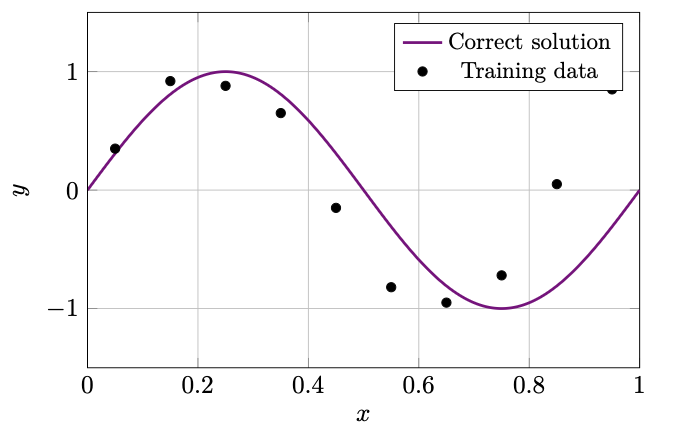
\includegraphics[width=0.8\textwidth]{images/polynomial_fitting_problem.png}
        \caption{Polynomia Fitting Problem: Data generated from \( sin(2\pi x) \) with noise}
    \end{figure}
\end{center}
\subsection{Model: Polynomial Functions}
\begin{definition}{Polynomia Model}
\centering 
We choose to model the data using polynomia functions:
\[
  f_w(x) = \sum_{j = 0}^{M} w_j x^j
\]
where:
\begin{itemize}
    \item \( M \) is the \textbf{degree of the polynomial} (a hyperparameter)
    \item \( w = \left\{w_0, \ldots, w_M \right\} \) are the \textbf{parameters} to be learned 
    \item The \textbf{hypotesis space} for a fixed degree \( M \) is: \( \mathcal{H}_M = \left\{ f_w : w \in \mathbb{R}^{M + 1} \right\} \)
\end{itemize}
\end{definition}
Different values of \( M \) give us different hypothesis spaces:
\begin{itemize}
    \item \( M = 0 \): Constant functions (horizontal lines)
    \item \( M = 1 \): Linear functions (straight lines)
    \item \( M = 2 \): Quadratic functions (parabolas)
    \item \( M = 3 \): Cubic functions 
    \item Higher \( M \): More complex curves
\end{itemize}
\subsection{Error function: Mean Squared Error}
To measure how well our polynomial fits the data, we use the Mean Squared Error (MSE):
\[
  E(f;\mathcal{D}_n) = \frac{1}{n} \sum_{i = 1}^{n} [f(x_i) - y_i]^2
\]
This error function:
\begin{center}
    \begin{figure}[H]
        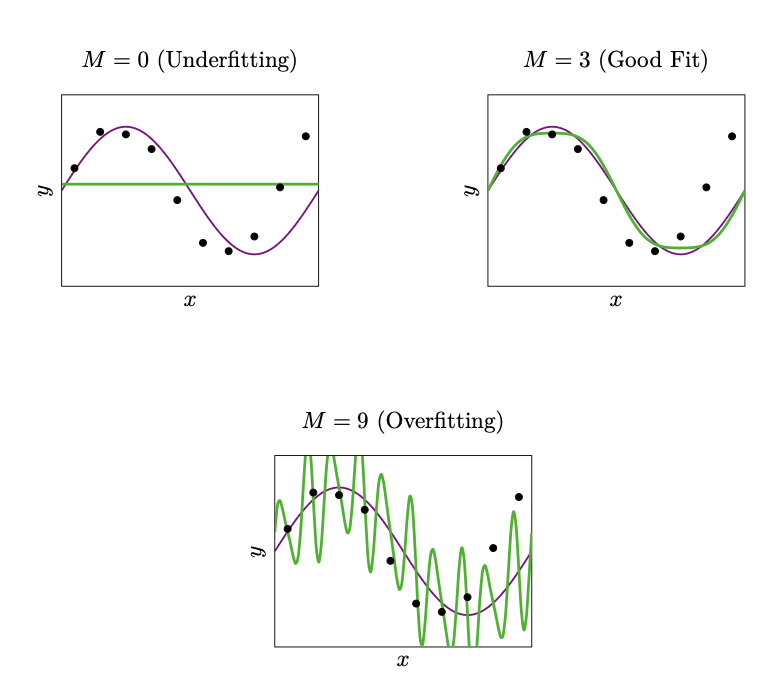
\includegraphics[width=0.9\textwidth]{images/polynomial_fits.png}
        \caption{Polynomial fits with different degrees: \( M = 0 \) (underfitting), \( M = 3 \) (good fits), \( M = 9 \) (overfitting). Purple: true function, Green: fitted polynomial, Black dots: training data}
    \end{figure}
\end{center}
\begin{itemize}
    \item Computes the squared difference between the prediction \( f(x_i) \) and the ground-truth label \( y_i \) for each point 
    \item Averages these squared differences over all \( n \) training points 
    \item Is also called a \textbf{pointwise loss} because it measures the error at each individual data point
\end{itemize}
The learning algorithm's goal is to find the parameters \( w \) that minimize this error function:
\[
  w^* = \text{ arg } \underset{w \in \mathcal{R}^{M + 1}}{\text{min}} E(f_w;\mathcal{D}_n)
\]
\textbf{Choice of Model Comlpexity is Crucial}:
\begin{itemize}
    \item Too small \( M \): Underfitting (cannot captuer pattern)
    \item Appropriate \( M \): Good fit (captures underlying pattern)
    \item Too large \( M \): Overfitting (fits noise, poor generalization)
\end{itemize}
\section{Underfitting and Overfitting}
\textbf{Two fundamental problems in ML}
\vspace{1em}
\noindent
\newline
Underfitting (too simple) \( \leftrightarrow \) Overfitting (too complex)
\vspace{1em}
\noindent
\newline
Two fundamental problems can occur when training machine learning models: underfitting and overfitting. Understanding these 
concepts is crucial for building models that generalize well.
\subsection{Definitions}
\begin{definition}{Underfitting}
\centering 
\textbf{Underfitting} is a scenario where a model is unable to capture the relationship between the input (x) and output (y) 
variables accurately, generating a high error rate on both the training set and unseen data (e.g., testing set).
\vspace{1em}
\noindent
\newline
The model is too simple and has not yet learned from the data. It performs poorly on both training and test data.
\end{definition}
\begin{definition}{Overfitting}
\centering 
\textbf{Overfitting} occurs when the model gives accurate predictions for training 
data (lower training error) but not for testing data (higher testing error).
\vspace{1em}
\noindent
\newline
The model is too sensitive to the training data and has essentially memorized it, including its noise 
and peculiarities, rather learning the underlying pattern.
\end{definition}
\subsection{The Bias-Variance Trade-off}
The relationship between model complexity, training error can be visualized as follows:
\begin{center}
    \begin{figure}[H]
        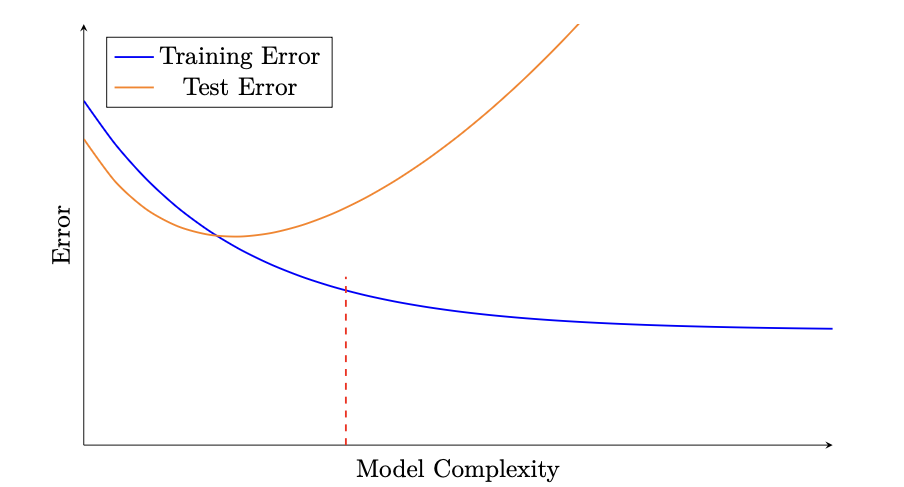
\includegraphics[width=0.9\textwidth]{images/model_complexity.png}
        \caption{Bias-Variance Trade-off: Training and Test Error vs. Model Complexity}
    \end{figure}
\end{center}
\begin{itemize}
    \item \textbf{Left side of the graph (low complexity)}: High error rate in both training and testing \( \rightarrow \) \textbf{Underfitting}
    \item \textbf{Middle Region (optimal complexity)}: Low error rate in both training and testing \( \rightarrow \) \textbf{Best Fit}
    \item \textbf{Right side of the graph (high complexity)}: Low error rate in training but high error rate in testing \( \rightarrow \) \textbf{Overfitting}
\end{itemize}
\subsection{Diagnostic Matrix}
We can dignose the state of our model by examining both training and test errors:
\begin{center}
    \begin{tabular}{ |c|c|c| }
        \hline
        & \textbf{Low training error} & \textbf{High training error} \\
        \hline 
        \textbf{Low Test Error} & OK (Goot fit) & Underfitting \\
        \hline 
        \textbf{High Test Error} & Overfitting & Underfitting \\
        \hline
    \end{tabular}
\end{center}
\subsection{How to handle onverfitting}
When the model is too sensitive to training data and overfits, we can apply several strategies:
\begin{enumerate}
    \item \textbf{Try a simpler model}: Use a model with fewer parameteres or lower complexity 
    \item \textbf{Try a less powerful model}: Choose a model architecture with reduced capacity 
    \item \textbf{Increase regularization impact}: Apply techniques that penalize model complexity:
    \begin{itemize}
        \item Early stopping: stop training before the model overfits 
        \item L1/L2 regularization: Add penalty terms to the loss function 
    \end{itemize}
    \item \textbf{Use a smaller number of features}:
    \begin{itemize}
        \item Remove some features that may be causing overfitting 
        \item Apply feature selection techniques to identify the most relevant features 
    \end{itemize}
    \item \textbf{Get more data}: Increasing the training set size helps the model learn more generalizable patterns
\end{enumerate}
\subsection{How to handle unverfitting}
When the model has not yet learned from the data and underfits, we can try:
\begin{enumerate}
    \item \textbf{Try more complex model}: Use models with larger number of parameters that can capture more intricate patterns 
    \begin{itemize}
        \item Ensemble learning: Combine multiple models 
    \end{itemize}
    \item \textbf{Less regularization}: Reduce or remove regularization constraints that may be limiting the model's capacity 
    \item \textbf{A larger quantity of features}: Add more features or engineer new features that better capture the underlying relationships (get more features)
\end{enumerate}
\subsection{Polynomial Fitting Example Revisited}
Let's examine how different polynomial degrees affect the fit:
\begin{itemize}
    \item \( M = 0 \) (constant function): Severe underfitting. The horizontal line cannot capture any of the sinusoidal pattern. Both training and validation errors are high 
    \item \( M = 1 \) (linear function): Still underfitting. A straight line cannot represent the curved pattern. Both errors remain high.
    \item \( M = 3 \) (cubic polynomial): Good fit. The model captures the underlying sinusoidal pattern well. Both training and validation errors are low, and the curves are similar 
    \item \( M = 9 \) (9th-degree polynomial): Overfitting. The model passes through alla training points (very low training error) but oscillates wildly between them. The validation error is high because the model has learned the noise rather than the signal.
\end{itemize}
The error plot shows:
\begin{itemize}
    \item \textbf{Training error} (blue line): Decresases monotonically as \( M \) increases 
    \item \textbf{Validation error} (orange line): Decreases initially, reaches a minimum around \( M = 3 \), then increases again 
    \item The optimal model complexity is where the validation error is minimized
\end{itemize}
\begin{center}
    \begin{figure}{H}
        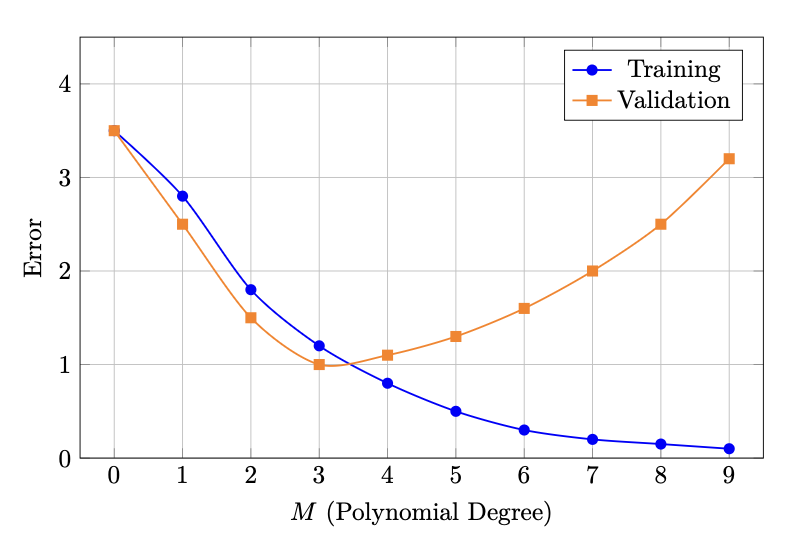
\includegraphics[width=0.9\textwidth]{images/polynomial_degree.png}
        \caption{Training and Validation Error vs. Polynomial Degree \( M \)}
    \end{figure}
\end{center}
\textbf{Key Insight}
\vspace{1em}
\noindent
\newline
Minimizing training error alone is \textbf{not sufficient}
\newline
Must monitor validation/test error for generalization 
\section{Regularization}
\textbf{One of the most important techinques in ML} \( \rightarrow \) Prevents overfitting and improves generalization 
\vspace{1em}
\noindent
\newline
Regularization is one of the most important techniques in machine learning to prevent overfitting and improve 
model generalization.
\subsection{What is Regularization?}
\begin{definition}{Regularization}
\centering 
Regularization refers to techniques that are used to calibrate machine learning 
models in order to minimize the adjusted loss function and prevent overfitting 
or underfitting.
\vspace{1em}
\noindent
\newline
In practice, regularization is a modification of the training error function by appending a term 
\( \omega(f) \) that typically penalizes complex solutions.
\end{definition}
\subsection{The regularized objective function}
The regularized objective function has the following form:
\[
  E_{reg} (f;\mathcal{D}_n) = E(f;\mathcal{D}_n) + \lambda_n \omega(f)
\]
where:
\begin{itemize}
    \item \( E(f;\mathcal{D}_n) \) is the \textbf{training error function} (e.g., MSE)
    \item \( \omega(f) \) is the \textbf{regularization term} that penalizes model complexity 
    \item \( \lambda_n \) is the \textbf{tradeoff hyperparameter} that controls the strngth of regularization
\end{itemize}
The regularization term acts as a penalty that discourages the model from becoming too complex.
By minimizing this combined objective, we find models that fit the data well while remaining relatively simple.
\subsection{Effect of Regularization}
The regularization term \( \omega(f) \) typically measures some notion of model complexity. When we minimize the regularized objective:
\begin{itemize}
    \item We balance fitting training data (low \(E(f;\mathcal{D}_n) \)) with keeping the model simple (low \( \omega(f) \))
    \item The hyperparameter \( \lambda_n \) controls this tradeoff 
    \item Higher \( \lambda_n \) means stronger regularization (simpler models)
    \item Lower \( \lambda_n \) means weaker regularization (more complex models allowed)
\end{itemize}
\subsection{Regularization in Polynomial Fitting}
For the polynomial fitting example, we can regularize by penalizing polynomials with large coefficients. The regularized error function becomes:
\[
  E_{reg} (f_w;\mathcal{D}_n) = \frac{1}{n} \sum_{i = 1}^{n}[f_w(x_i) - y_i]^2 + \frac{\lambda}{n} \parallel w \parallel^2
\]
where:
\begin{itemize}
    \item The fisrt term is the training erorr (MSE)
    \item \( \frac{\lambda}{n} \parallel w \parallel^2 = \frac{\lambda}{n} \sum_{j = 0}^{M} w_{j}^2 \) is the regularization term (L2 regularization)
    \item \( \lambda \) is the tradeoff hyperparameter
\end{itemize}
\subsubsection{Effect of the Regularization Parameter \( \lambda \)}
The choice of \( \lambda \) significantly affects the model:
\begin{itemize}
    \item \( \lambda \approx 10^{-18} \) (\textbf{very small}): Almost no regularization. The model can have large coefficients 
        and may overfit. The polynomial fits the training data very closely, including noise.
    \item \( \lambda = 1 \) (\textbf{moderate}): Balanced regularization. The model is penalized for having large coefficients, leading to amoother curve that generalizes better. This often provides the best tradeoff between training and validation error.
    \item \( \lambda \) \textbf{very large}: Strong regularization. The penalty for large coefficients is so high that the model becomes too simple and may underfit. The curve becomes nearly flat.
\end{itemize}
\subsubsection{Regularization Path}
The plot of error vs. \( ln(\lambda) \) shows:
\begin{itemize}
    \item \textbf{Left side (small \( \lambda \))}: Low training error, high validation error \( \rightarrow \) Overfitting 
    \item \textbf{Middle region:} Both errors are low \( \rightarrow \) Good fit
    \item \textbf{Right side (large \( \lambda \))}: Both errors increase \( \rightarrow \) Underfitting
\end{itemize}
The optimal \( \lambda \) is found where the validation error is minimized.
\begin{center}
    \begin{figure}[H]
        \centering 
        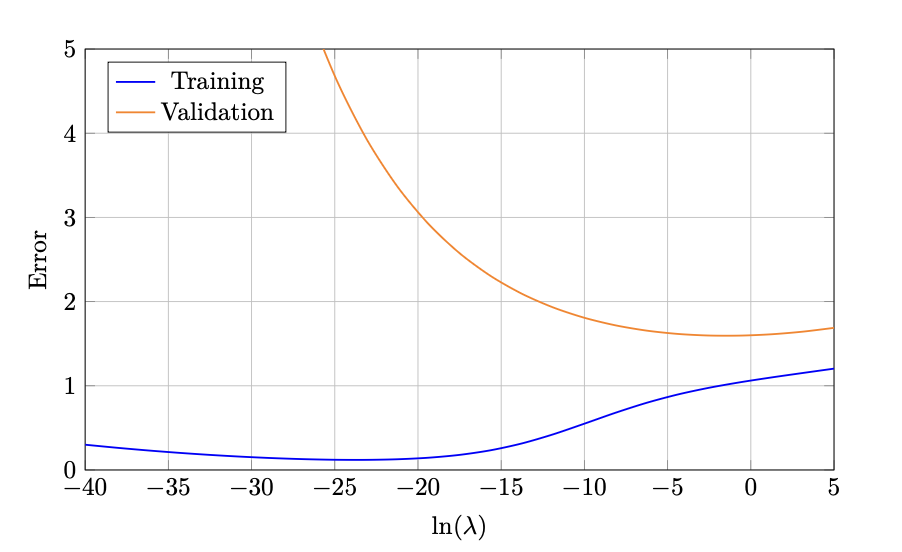
\includegraphics[width=0.9\textwidth]{images/ln.png}
        \caption{Training and Validation Error vs. \( ln(\lambda) \) (Regualarization Strength)}
    \end{figure}
\end{center}
\subsection{Generalization and Data Size}
An important theoretical result in machine learning relates training erorr to generalization error:
\begin{theorem}{Generalization with Infinite Data}
\centering
\textit{As the number of training samples approaches infinity, the training error approzimates the generalization erorr}:
\[
  E(f;\mathcal{D}_n) \rightarrow E(f;p_{data}) \text{ as } n \to \infty 
\]
\end{theorem}
This means:
\begin{itemize}
    \item With a small dataset (\( n = 15 \)), even a complex model \( (M = 9) \) may overfit because there isn't enough data to constrain the parameters
    \item With a large dataset \( (n = 100) \), the same complex model can generalize well beacouse the abundant data prevents overfitting 
    \item More data allows us to use more complex models without overfitting
\end{itemize}
\textbf{Visual example}:
\begin{itemize}
    \item \( n = 15, M = 9 \): The 9th-degree polynomial overfits, oscillating widly between the few training points 
    \item \( n = 100, M = 9 \): With 100 training points, the same 9th-degree polynomial fits smoothly and generalizes well
\end{itemize}
\textit{"Get mora data" is often the most effective solution to overfitting}. With sufficinet data, even complex models can generalize well.
\begin{center}
    \begin{figure}
        \centering
        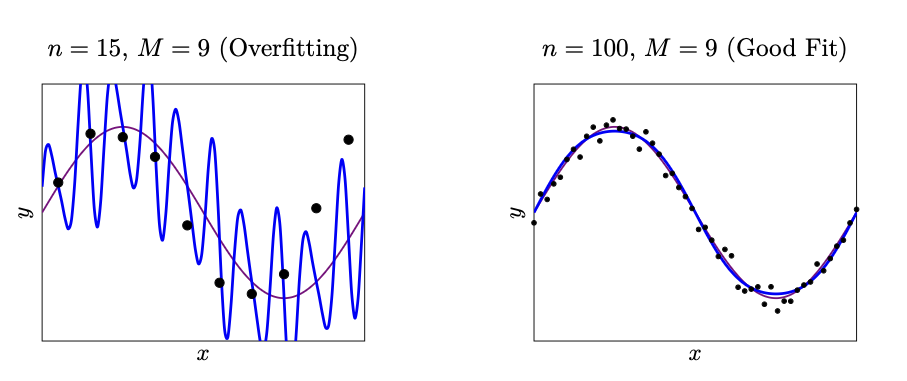
\includegraphics[width=0.9\textwidth]{images/overfitting.png}
        \caption{Effect of data size on generalization: With fex data points \( (n = 15) \), a complex model 
    \( (M = 9) \) overfits. With many data points \( (n = 100) \), the same model generalizes well. Purple: 
    true function, Blue: fitted polynomial, Black dots: trining data.}
    \end{figure}
\end{center}

\part{Model Evaluation and Regression Methods}
\section{Model evaluation for Classification and Regression}
\subsection{Recap: Train, Validation, and Test Sets}
The machine learning workflow involves three distinct datasets, each serving a specific purpose:
\subsubsection{The three dataset}
\begin{enumerate}
    \item \textbf{Training set}: Used to train the machine learning algorithm 
    \begin{itemize}
        \item The model learns patterns and relationships from this data 
        \item Parameters are optimized to minimize training error 
    \end{itemize}
    \item \textbf{Validation set}: Used during the learning phase 
    \begin{itemize}
        \item Also called the \textit{mini test set}
        \item Helps select the better performing algorithm among alternatives 
        \item Used to tune hyperparameters of the model 
        \item Provides feedback to adjust the model before final testing
    \end{itemize}
    \item \textbf{Test set}: User for final model evaluation 
    \begin{itemize}
        \item Provides an unbiased assessment of model perfromance 
        \item The model has never seen this data during training or validation 
        \item Tells us how well the model will perform on new, real-world data
    \end{itemize}
\end{enumerate}
\subsection{The importance of the validation set}
The validation set plays crucial role in the machine learning pipeline and must kept \textbf{separate from the training set}.
\begin{center}
    \begin{figure}[H]
        \centering 
        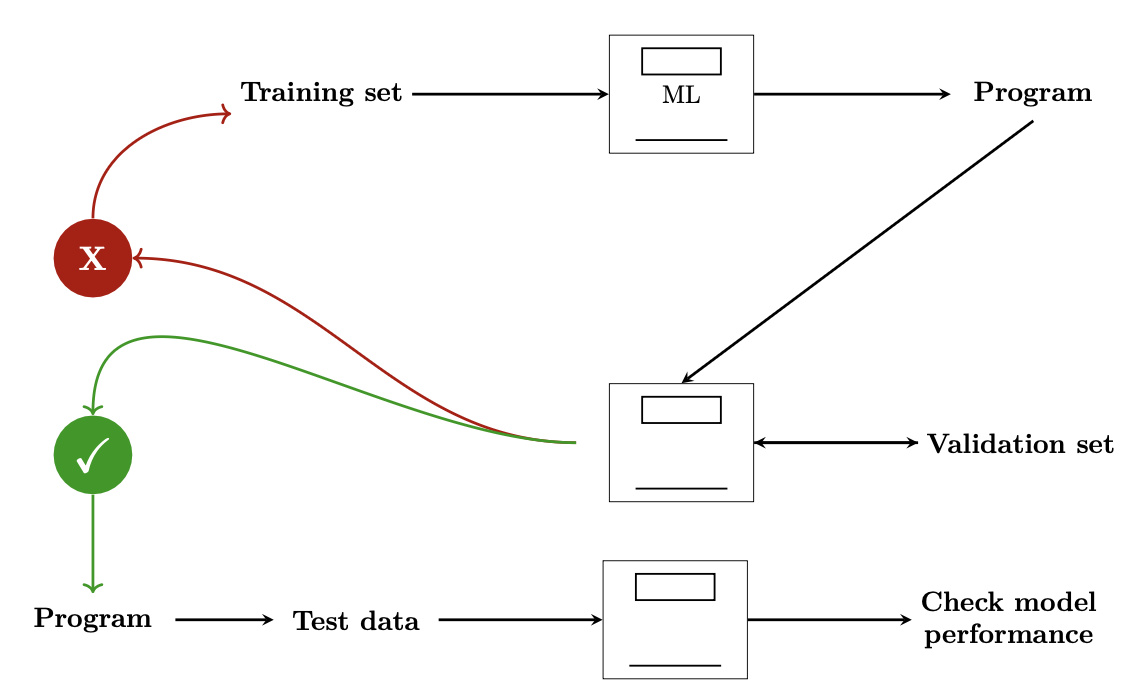
\includegraphics[width=0.9\textwidth]{images/workflow.png}
        \caption{Machine learning workflow. Training set trains the model, validation set evaluates 
        and provides feedback (thumbs down = retain, thumbs up = proceed to testing), test set checks final perfromance}
    \end{figure}
\end{center}
\subsubsection{Why separate the validation set?}
The validation set is used for two main purposes:
\begin{enumerate}
    \item \textbf{Algorithm Selection}: To pick the better performing algorithm 
    \begin{itemize}
        \item Compare different model architectures (e.g., decision trees vs. neural networks)
        \item Select the model that performs best on unseen data
    \end{itemize}
    \item \textbf{Hyperparameter Tuning}: To decide the hyperparameters of an algorithm 
    \begin{itemize}
        \item Hyperparameters are configuration setting that are not learned from data
        \item Examples: learning rate, regularization strength \( (\lambda) \), number of layers, tree depth 
        \item The validation set helps find the optimal hyperparameter values
    \end{itemize}
\end{enumerate}
\textit{Note}. \textbf{ATTENTION}: Splitting the datasets into training and validation sets can be done 
randomly to avoid bias. However, tehre are some \textbf{specific rules} to apply when performing this 
split to ensure reliable model evaluation.
\subsection{Specific Rules for Dataset Splitting}
When splitting data into training, validation, and testing sets, you can have conflicting priorities.
The key is to balance these priorities appropriately.
\subsubsection{Priority 1: Accurate Error Estimation}
\textbf{Goal}: Estimate future error (i.e., validation/testing error) as accurately as possible.
\begin{center}
    \begin{figure}[H]
        \centering 
        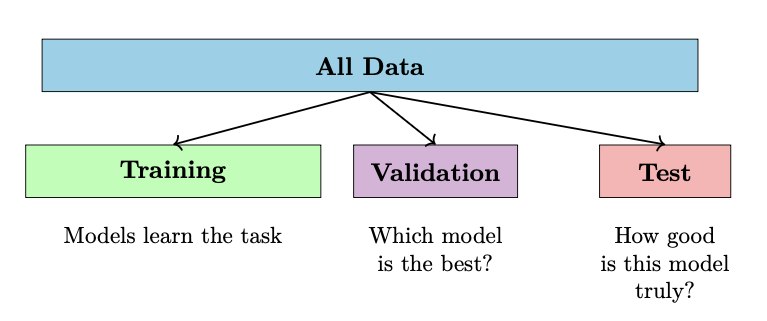
\includegraphics[width=0.9\textwidth]{images/dataset_splitting.png}
        \caption{Dataset splitting: Training for learning, Validation for model selection, Test for final evaluation}
    \end{figure}
\end{center}
\textbf{How to achieve this}: By making the \textbf{validation set as big as possible}.
\vspace{1em}
\noindent
\newline
\textit{(High confidence interval)}
\begin{itemize}
    \item A larger validation set provides more reliable error estimates 
    \item Reduces variance in performance metrics 
    \item Gives higher confidence that the measured perfromance reflects true generalization
\end{itemize}
\subsubsection{Priority 2: Accurate Classifier Learning}
\textbf{Goal}: Learn classifier as accurately as possible.
\vspace{1em}
\noindent
\newline
\textbf{How to achieve this}: By making the \textbf{training set as big as possible}
\vspace{1em}
\noindent
\newline
\textit{(Better estimates, maybe better generalization)}
\begin{itemize}
    \item More training data allows the model to learn more robust patterns 
    \item Reduces overfitting by providing diverse examples 
    \item Generally leads to better generalization on unseen data
\end{itemize}
\subsubsection{The critical Rule}
\textbf{CRITICAL REQUIREMENT} \( \rightarrow \) Training and validation/testing instance \textbf{CANNOT OVERLAP !!!}
\begin{itemize}
    \item If the same data appears in both training and validation/test sets, the evaluation is invalid 
    \item The model would be tested on data i has already seen during training 
    \item This lead to overlay optimistic performance estimates that don't reflect real-world performance 
    \item Data leakage between sets is one of the most common mistakes in machine learning
\end{itemize}
\textit{Observation}. The split between training and validation/test sets represents a fundamental trade-off:
\begin{itemize}
    \item Larger training set \( \rightarrow \) Better model learning, but less reliable error estimation 
    \item Larger validation/test set \( \rightarrow \) More reliable error estimation, but potentially worse model learning
\end{itemize}
Common splits include 70-15-15, 80-10-10, or 60-20-20 (train-validation-test), depending on the 
total dataset size and specific requirements.
\section{Cross Validation}
\subsection{When do we need Cross Validation?}
In cases where we don't have enough data to randomly split between training
(e.g., 60\% of the totale data), validation (e.g., 20\% of the data), and testing 
(e.g., 20\% of the totale data), we need to use \textbf{cross-validataion}.
\begin{definition}{Cross Validation}
\centering Cross-Validation is a resampling technique that involves reusing 
a portion of the training set itself to validate performance by retraining not just one,
but \( N \) models.    
\end{definition}
\subsection{Key characteristics of Cross Validation}
\begin{itemize}
    \item \textbf{Multiple models}: Cross-Validation involves training \( N \) models instead of just one 
    \item \textbf{Computional cost}: Performing cross-validation requires \( N \) training sessiones and can be more computationally demanding 
    \item \textbf{Better use of limited data}: When data is scarce, cross-validation, allows us to use the available data more efficently for both training and validation
\end{itemize}
\subsection{Fundamental Rules of Cross Validation}
Cross validation must respect certain constraints to ensure valid model evaluation:
\begin{enumerate}
    \item \textbf{No overlap}: Training and validation cannot overlap, but \( n_{train} + n_{validation} \) = constant 
    \item \textbf{Each instance used once per fold}: At each fold (step), you use each instance only in one set, so there is no overlapping within signle fold 
    \item \textbf{Every sample participates}: Every sample is in both training and testing but not at the same time 
    \begin{itemize}
        \item This reduces the changs of getting a biased training set 
        \item Ensures all data contributes to both training and validation across different folds
    \end{itemize}
\end{enumerate}
\subsection{K-Fold Cross Validation}
K-fold cross validation is the most common form of cross validation, where the dataset is divided into \( k \) equal parts (folds).
\subsubsection{How K-Fold Cross Validation works}
In the case of k-fold cross-validation:
\begin{enumerate}
    \item We split out dataset into \( k \) groups (folds)
    \item We perform training \( k \) times on \( (N/k)(k - 1) \) data points 
    \item We measure performance on the last \( N/k \) data points (the validation fold)
    \item Our cross-validation performance will be the \textbf{average of the perfromance of the} \( k \) \textbf{tests}
\end{enumerate}
\textit{Note}. \textbf{Important constraint}: Training set and validation set cannot overlap, but the sum of training and validation 
data is constant (the totale dataset size).
\subsubsection{Visual Representation of K-Fold Cross Validation}
\begin{center}
    \begin{figure}[H]
        \centering
        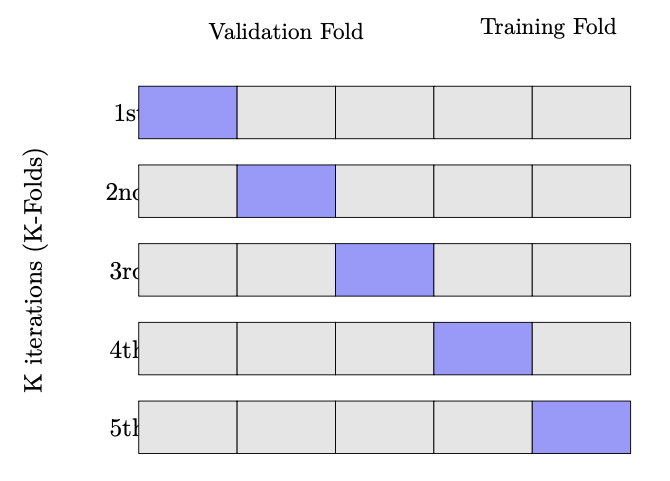
\includegraphics[width=0.8\textwidth]{images/k-fold.png}
        \caption{K-Fold Cross Validation: Each row represents on iteration where a different fold serves as validation (blue) while the rest serve as training (gray)}
    \end{figure}
\end{center}
\subsection{Example: 5-Fold Cross Validation}
Let's examine a concrete example with 5 folds:
\begin{itemize}
    \item \textbf{Step 1}: Randomly split the data into 5 folds 
    \item \textbf{Step 2}: Test on each fold while training on 4 other folds (80\% train, 20\% test)
    \item \textbf{Step 3}: Average the results over 5 folds
\end{itemize}
\begin{center}
    \begin{figure}[H]
        \centering
        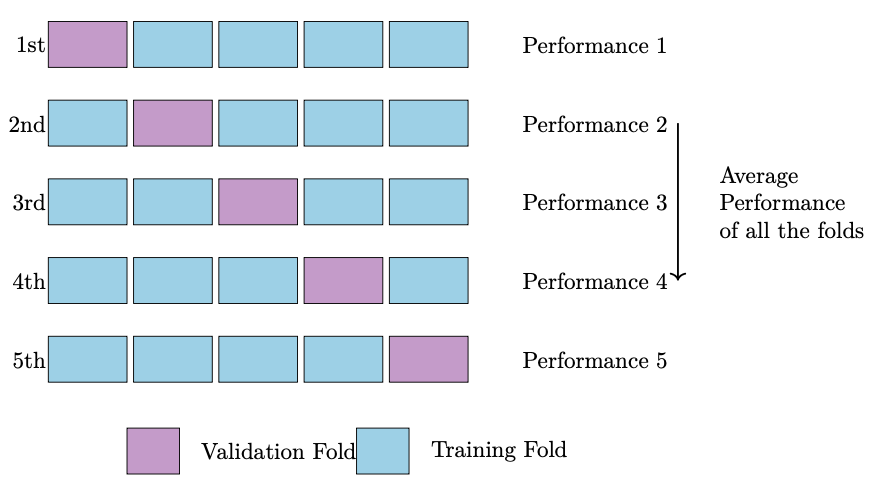
\includegraphics[width=0.8\textwidth]{images/5-fold.png}
        \caption{5-Fold Cross Validation Example: Each fold serves as validation once, and the final perfromance is the average of all 5 iterations}
    \end{figure}
\end{center}
\subsubsection{The process in Detail}
For each of the 5 iterations:
\begin{enumerate}
    \item \textbf{Iteration 1}: Use fold 1 as validation, folds 2-5 as training \( \rightarrow \) Get Performance 1 
    \item \textbf{Iteration 2}: Use fold 2 as validation, folds 1,3-5 as training \( \rightarrow \) Get Performance 2
    \item \textbf{Iteration 3}: Use fold 3 as validation, folds 1-2,4-5 as training  \( \rightarrow \) Get Performance 3 
    \item \textbf{Iteration 4}: Use fold 4 as validation, folds 1-3,5 as training  \( \rightarrow \) Get Performance 4 
    \item \textbf{Iteration 5}: Use fold 5 as validation, folds 1-4 as training  \( \rightarrow \) Get Performance 5
\end{enumerate}
\textbf{Final Cross-Validation Performance}:
\[
  \text{CV Performance } = \frac{1}{5} \sum_{i = 1}^{5} \text{ Performance}_i
\]
\subsection{Advantages of Cross Validation}
\begin{itemize}
    \item \textbf{Better use of limited data}: Every data point is used for both training and validation 
    \item \textbf{More reliable performance estimates}: Averaging over multiple folds reduces vairance in the performance estimate 
    \item \textbf{Reduces bias}: Every sample participates in validation, reducing the risk of biased validation set 
    \item \textbf{Detects overfitting}: If performance varies significantly across folds, it may indicate overfitting or data quality issues
\end{itemize}
\subsection{Disadvantages of Cross Validation}
\begin{itemize}
    \item \textbf{Computationally expensive}: Requires training \( k \) models instead of one 
    \item \textbf{Time-consuming}: Training time is multiplied by the number of folds 
    \item \textbf{Not suitable for very large datasets}: When a data is abundant, a simple train-validation-test split is more efficient
\end{itemize}
\textit{Observation}. The choice of \( k \) (number of folds) involves a tradeoff:
\begin{itemize}
    \item \textbf{Larger} \( k \): More accurate performance estimate, but more computationally expensive 
    \item \textbf{Smaller}: \( k \): Faster computation, but less reliable performance estimate 
    \item Common choices: \( k = 5 \) or \( k = 10 \).
    \item Extreme case: \( k = N \) (Leave-One-Out Cross Validation) uses each single sample as validation once
\end{itemize}
\section{Leave-One-Out Cross Validation}
\subsection{What is Leave-One-Out Cross Validation?}
Leave-One-Out Cross Validation (LOOCV) is an extreme case of k-fold cross validation that is particularly useful when we have 
very few data points.
\begin{definition}{Leave-One-Out Cross Validation}
\centering 
LOOCV is \( n \)-fold cross validation where \( n \) equals the total number of samples.
In each iteration, we train on all \( (n - 1) \) samples and test on exactly 1 instance.
\end{definition}
\subsection{How LOOCV Works}
The process involves:
\begin{enumerate}
    \item Take the entire dataset of \( n \) samples
    \item For each sample \( i \) (where \( i = 1,2, \ldots, n) \):
    \begin{itemize}
        \item Use sample \( i \) as the validation set (1 sample)
        \item Use all other samples \( (n - 1) \) as the training set 
        \item Train the model and evaluate on the single validation sample
    \end{itemize}
    \item Repeat this process \( n \) times (once for each sample)
    \item Average the performance across all \( n \) expriments
\end{enumerate}
\begin{center}
    \begin{figure}[H]
        \centering 
        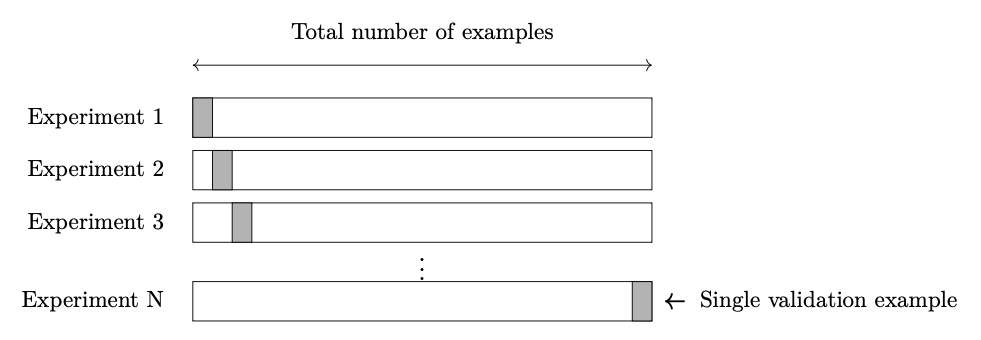
\includegraphics[width=0.8\textwidth]{images/leave-one.out.png}
        \caption{Leave-One-Out Cross Validation: Each experiment uses exactly one sample for validation (gray) and all others for training (white)}
    \end{figure}
\end{center}
\subsection{Pros and Cons of LOOCV}
\subsubsection{Advantages}
\begin{itemize}
    \item \textbf{Best possible classifier}: The model is learned from \( n - 1 \) training examples, which is the maximum possible training data 
    \item \textbf{Maximizes training data}: Each model uses almost all available data for training 
    \item \textbf{Unbiased estimate}: Provides a nearly unbiased estimate of model performance 
    \item \textbf{Deterministic}: No randomness in the splitting process (every sample is used exactly once as validation)
\end{itemize}
\subsubsection{Disadvantages}
\begin{itemize}
    \item \textbf{High computational cost}: Must re-learn everything for \( n \) times, where \( n \) is the total number of samples 
    \item \textbf{Time-consuming}: For large datasets, LOOCV becomes impratical 
    \item \textbf{High variance}: Performance estimates can have high variance, especially with small datasets
\end{itemize}
\textit{Note}. LOOCV is most appropriate when:
\begin{itemize}
    \item The dataset is very small (e.g., \( n < 50 \)) 
    \item Computational resources are available 
    \item You need the most accurate performance estimate possible
\end{itemize}
For larger datasets, standard k-fold cross validation (with \( k = 5 \) or \( k = 10 \)) is typically preferred 
due to its better balance between computation cost and performance estimation accuracy.
\section{Stratification in Cross Validation}
\subsection{The problem: Imbalanced Classes}
In many real-world datasets, class labels are not evenly distributed. For example, in a medica 
diagnosis dataset, healthy patients might vastly outnumber sick patients. When performing cross validation on such 
imbalanced datasets, random splitting can lead to folds with very different calss 
distribution.
\subsection{What is Stratification?}
\begin{definition}{Stratification}
\centering 
Stratification is a technique to keep class labels \textbf{balanced across training and validation sets} during 
cross validation. Instead of randomly diving the dataset, we ensure that each fold maintains approximately the same proportion 
of samples for each class as the complete dataset. 
\end{definition}
\subsection{How Stratified K-Fold Works}
The stratification process works as follows:
\begin{enumerate}
    \item \textbf{Divide by class}: Instead of taking the dataset and dividing it randomly into \( K \) parts, take the dataset and divide it into individual classes 
    \item \textbf{Split each class}: Then for each class, divide the instances into \( K \) parts 
    \item \textbf{Assemble folds}: Assemble the \( i \)-th part from alla classes to make the \( i \)-th fold 
    \item \textbf{Important}: It still random! The splitting within each class is random, but the proportions are maintained
\end{enumerate}
\subsection{Example: Stratified 5-Fold Cross Validation}
Let's consider a concrete scenario with an imbalanced dataset containing 300 samples, divided into three classes 
(A, B, and C), where Class A has more samples than the other two.
\subsubsection{Imbalanced Dataset}
\begin{itemize}
    \item \textbf{Class A}: 200 samples \( (66.7\%) \).
    \item \textbf{Class B}: 50 samples \( (16.7\%) \).
    \item \textbf{Class C}: 50 samples \( (16.7\%) \).
    \item \textbf{Total}: 300 samples
\end{itemize}
\subsubsection{Split the Dataset into Five Folds with Stratification}
Each fold will have 60 samples total, maintaining the class proportions:
\begin{itemize}
    \item \textbf{Fold 1}: 60 samples (Class A: 40, Class B: 10, Class C: 10)
    \item \textbf{Fold 2}: 60 samples (Class A: 40, Class B: 10, Class C: 10)
    \item \textbf{Fold 3}: 60 samples (Class A: 40, Class B: 10, Class C: 10)
    \begin{center}
        \begin{figure}[H]
            \centering 
            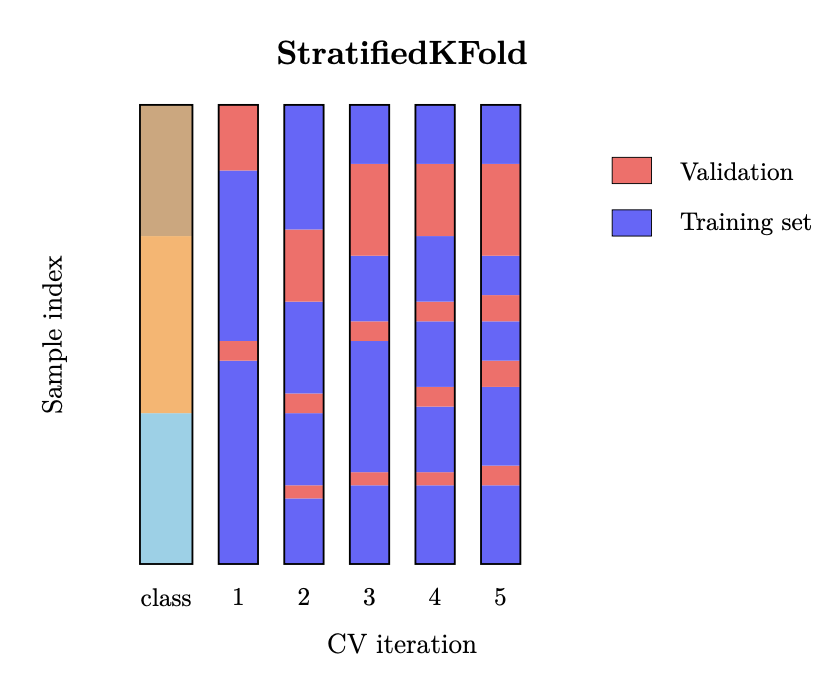
\includegraphics[width=0.8\textwidth]{images/stratified.png}
            \caption{Stratified K-Fold: Each fold maintains the same class proportions across all folds}
        \end{figure}
    \end{center}
    \item \textbf{Fold 4}: 60 samples (Class A: 40, Class B: 10, Class C: 10)
    \item \textbf{Fold 5}: 60 samples (Class A: 40, Class B: 10, Class C: 10)
\end{itemize}
Notice that each fold maintains the same \( 66.7\%-16.7\%-16.7\% \) class distribution as the original dataset.
\subsubsection{Train and Validate}
The cross-validations proceeds as follows:
\begin{enumerate}
    \item \textbf{Iteration 1}: Train on Folds 1, 2, 3, and 4, Validate on Fold 5 
    \item \textbf{Iteration 2}: Train on Folds 2, 3, 4, and 5, Validate on Fold 1 
    \item \textbf{Iteration 3}: Train on Folds 1, 3, 4, and 5, Validate on Fold 2
    \item \textbf{Iteration 4}: Train on Folds 1, 2, 4, and 5, Validate on Fold 3 
    \item \textbf{Iteration 5}: Train on Folds 1, 2, 3, and 5, Validate on Fold 4
\end{enumerate}
\subsubsection{Average the performance Metrics}
\begin{itemize}
    \item Calculate performance metrics for each iteration 
    \item Average these metrics to evaluate the model's performance robustly 
\end{itemize}
\subsection{Why Stratification Matters}
\begin{itemize}
    \item \textbf{Prevents biased folds}: Without stratification, some folds might have very few (or no) examples of minority classes 
    \item \textbf{Consistent evaluation}: Each fold represents the overall dataset distribution, leading to more reliable performance estimates 
    \item \textbf{Better for imbalanced datasets}: Particularly important when dealing with class imbalance 
    \item \textbf{Reduces variance}: Performance estimates have lower variance across folds
\end{itemize}
\textit{Note}. \textbf{When to use stratification}:
\begin{itemize}
    \item Always use stratification for classification problems with imabalanced classes 
    \item It's generally a good practice even for balanced datasets 
    \item Most machine learning librearies (e.g., scikit-learn) provide stratified cross-validation functions 
    \item For regression problems, stratification is not applicable (since there are no discrete classes)
\end{itemize}
\textbf{Observation}. Stratification ensures that:
\begin{itemize}
    \item Each fold is a good representative of the whole dataset
    \item Minority classes are adequately represented in both training and validation sets 
    \item Performance metrics are more stable and reliable across folds 
    \item The model ses a balanced distribution of classes during each training iteration
\end{itemize}
\section{Evaluation Measures}
Once we have trainend out models and performed cross-validation, we need to evaluate their performance.
Different tasks require different evaluation metrics.
\subsection{Why do we need Evaluation Measures?}
Evaluation measures serve two primary purpose:
\begin{enumerate}
    \item \textbf{To decide if our model is performing well}: Assess wether the model meets the requirements for the task 
    \item \textbf{To decide out of many models, which one performs better than the other}: Compare different models and select the best one for deployement
\end{enumerate}
\subsection{Evaluation Measures by Task Type}
Different nachine learning tasks require different evaluation approaches:
\subsubsection{Classification}
\textbf{Question}: How often does our model classify something right/wrong? 
\vspace{1em}
\noindent
\newline
Classification metrics measure the correctness of predictions, focusing on whether the predicted class matches the actual class.
\subsubsection{Regression}
\textbf{Question}: How close our model to what we are trying to predict?
\vspace{1em}
\noindent
\newline
Regression metrics measure the distance or error between predicted continuos values and avtual values.
\subsubsection{Clustering}
\textbf{Question}: How well does our model describe our data?
\vspace{1em}
\noindent  
\newline
Clustering evaluation is generally very hard because there's often no ground truth to compare 
against. Metrics must assess the quality of discovered patterns.
\section{Evaluation Measures of Classification}
\subsection{Types of Classification Problems}
A classification model takes a set of features as input and produces one or more classes as output.
\begin{definition}{Classification Type}
\centering Classification can be categorized into different types based on the number of classes:
\begin{itemize}
    \item \textbf{Binary classification}: In the case of two classes (0/1) or one vs rest (e.g., apples vs other fruits)
    \item \textbf{Multi-class Classification}: In the case having \( N \) classes to choose from (e.g., cat, dog, wolf, etc.)
    \item \textbf{Multi-label Classification}: A problem where an example can belong to multiple calsses simultaneously
\end{itemize}
\end{definition}
\subsection{The confusion matrix}
The confusion matrix is a fundamental tool for evaluating binary classification models. It provides a complete
picture of how the model perfrom across different types of predictions 
\subsubsection{Confusion Matrix for Binary classification}
\begin{center}
    \begin{figure}[H]
        \centering
        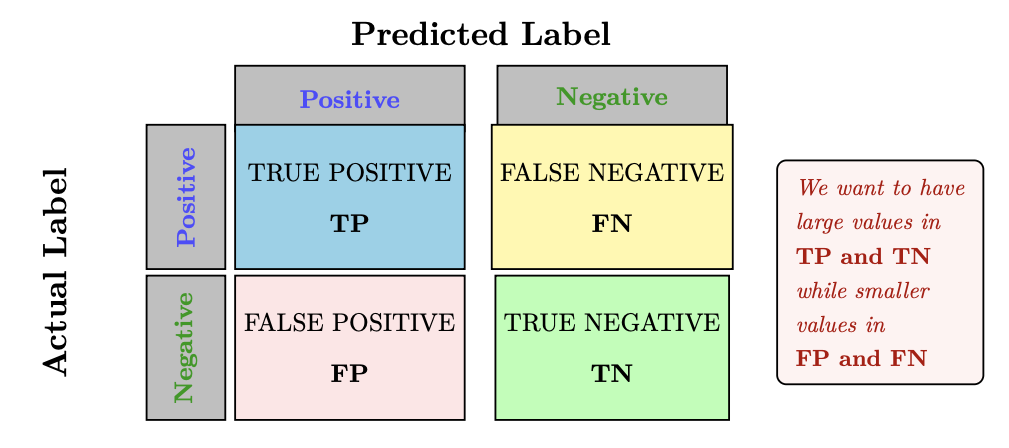
\includegraphics[width=0.8\textwidth]{images/confusion-matrix.png}
        \caption{Confusion Matrix for Binary Classification}
    \end{figure}
\end{center}
\subsubsection{Understanding the Confusion Matrix}
The confusion matrix has four components:
\begin{itemize}
    \item \textbf{True Positive (TP)}: The model correctly predicted the positive class
    \begin{itemize}
        \item Actual label: Positive
        \item Predicted label: Positive 
        \item \textcolor{blue}{Good prediction!}
    \end{itemize}
    \item \textbf{True Negative (TN)}: The model correctly predicted the negative class 
    \begin{itemize}
        \item Actual label: Negative
        \item Predicted label: Negative
        \item \textcolor{green}{Good Prediction!}
    \end{itemize}
    \item \textbf{False Positive (FP)}: The model incorrectly predicted positive (Type I error)
    \begin{itemize}
        \item Actual label: Negative 
        \item Prediction label: Positive 
        \item \textcolor{red}{Bad prediction!} (False alarm)
    \end{itemize}
    \item \textbf{False Negative (FN)}: The model incorrectly predicted negative (Type II error)
    \begin{itemize}
        \item Actual label: Positive 
        \item Prediction label: Negative 
        \item \textcolor{red}{Bad prediction!} (Missed detection)
    \end{itemize}
\end{itemize}
\textit{Note}. \textbf{Goal}: We want to maximize TP and TN (correct predictions) while miniimzing FP and FN (incorrect predictions).
\subsection{Classification Error and Accuracy}
From the confusion matrix, we can derive several important metrics.
\subsubsection{Classification error}
\begin{definition}{Classification Error}
\centering The classification error (also called misclassification rate) measures 
the proportion of incorrect predictions:
\[
  \text{Classification Error } = \frac{FP + FN}{TP + TN + FP + FN}
\]
This represent the fraction of all predictions that were wrong
\end{definition}
\subsubsection{Accuracy}
\begin{definition}{Accuracy}
\centering Accuracy measures the proportion of correct predictions:
\[
  \text{Accuracy } = 1 - \text{Error} = \frac{TP + TN}{TP + TN + FP + FN}
\]
This represent the fraction of all predictions that were correct
\end{definition}
\subsection{The problem with Accuracy: Imbalanced Classes}
While accuracy is a basic measure of "goodness" of a classifier, it can be very misleading 
when dealing with imbalanced classes.
\vspace{1em}
\noindent
\newline
\textbf{ATTENTION!} \( \rightarrow \) Accuracy is \textbf{very misleading} if we have \textbf{imbalanced classes}
\subsubsection{Example: The imablanced Dataset Problem}
Consider a dataset with severe class imbalance:
\begin{itemize}
    \item 90 samples for class "NO"
    \item 10 samples for class "YES"
\end{itemize}
\textbf{Native strategy}: A trivial classifier that predicts "NO" for every sample would achieve:
\[
  \text{Accuracy } = \frac{90}{100} = 90\%
\]
\textbf{The problem}: Despite having \( 90\% \) accuracy, this model is completely useless! It cannot 
classify any data belonging to the "YES" class. The model has learned nothing meaningful about the data.
\vspace{1em}
\noindent
\newline
\textit{Observation}. The example illusatrate why accuracy alone is insufficient for evaluating classifiers,
especially with imablanced dataset. We need additional metrics that provide a more nuanced view of model 
performance across all classes.
\vspace{1em}
\noindent
\newline
\textit{Note}. When dealing with imbalanced dataset, always consider:
\begin{itemize}
    \item Using stratified cross-validation 
    \item Examining the confusion matrix in detail
    \item Using additional metrics beyond accuracy (precision, recall, F1-score)
    \item Considering class-specific performance 
    \item Using techniques like oversampling, undersampling, or class weights
\end{itemize}
\subsection{Misses and False Alarms}
Beyond accuracy, we need more specific metrics to understand model performance. These metrics focus on different aspects of classification
errors.
\subsubsection{False Alarm Rate (False Positive Rate)}
\begin{definition}{False Alarm Rate = False Positive Rate}
\centering
\[
  \frac{FP}{FP + TN}
\]
This represents the \textit{percentage of negative samples we misclassified as positive}
\end{definition}
\subsubsection{Miss Rate (False Negative Rate)}
\begin{definition}{Miss Rate = True Positive Rate}
\centering 
\[
  \frac{TP}{TP + FN}
\]
This represent the \textit{percentage of positive samples we misclassified as negative}
\end{definition}
\subsubsection{Recall (True Positive Rate)}
\begin{definition}{Recall = True Positive Rate}
\centering 
\[
  \frac{TP}{TP + FN}
\]
This represent the \textit{percentage of positive samples we classified correctly}
\end{definition}
It also know as \textbf{Sensitivity} and can be expressed as: Recall = 1 - Miss Rate
\vspace{1em}
\noindent
\newline
\textit{Observation}. Recall answers the question: "Of all the actual positive cases, how many did we identity?"
\subsubsection{Precision}
\begin{definition}{Precision}
\centering 
\[
  \frac{TP}{TP + FP}
\] 
This represent the \textit{percentage positive out of what we predicted was positive}.
\vspace{1em}
\noindent
\newline
\textit{Observation}. Precision answer the question: "Of all the cases
we predicted as positive, how many were actually positive?"
\end{definition}
\subsection{Cost of the Task}
In pratice, we typically do not use evaluation mertics like accuracy, recall, 
or precision alone. Instead, we declare a combination of them together based on the specific 
requirements of the task
\subsubsection{The need for a single evaluation measure}
\begin{itemize}
    \item In oreder to optimize a learner automatically (i.e., during training), we need a \textbf{single evaluation measure}
    \item How do we decide that single metric?
    \begin{itemize}
        \item \textbf{Domain specific!} - It depends on the task
    \end{itemize}
\end{itemize}
\subsubsection{weighting Errors by Cost}
Depending on the \textbf{cost of the task}, we can decide whether we take 
more about having:
\begin{itemize}
    \item \textit{Less false positives}, or
    \item \textit{Less false negatives}
\end{itemize}
This is achieved through wighting them:
\[
  \text{Cost} = C_{FP} \times \text{FP } + C_{FN} \times \text{FN}
\]
where \( C_{FP} \) and \( C_{FN} \) are the costs associated with false positive and false negatives, respectively.
\begin{example}{Medical Diagnosis (Cancer detection)}
\centering 
\begin{itemize}
    \item False Negative (missing a cancer diagnosis): Very high cost - patient doesn't receive treatment 
    \item False Positive (false alarm): Lower cost - patient undergoes additional tests 
    \item Therefore: \( C_{FN} \gg C_{FP} \), we prioritize high recall
\end{itemize}    
\end{example}
\begin{example}{Spam Email Filter}
\centering 
\begin{itemize}
    \item False Positive (marking important email as spam): High cost - user misses important messages 
    \item False Negative (spam gets through): Lower cost - minore annoyance 
    \item Therefore: \( C_{FP} > C_{FN} \) we prioritize high precision
\end{itemize}
\end{example}
\subsection{F-Measure (F1 Score)}
The F-Measure combines precision and recall into a single metric, providing a balance between 
the two.
\begin{definition}{F1}
\centering The \textbf{F1 Score} is the harmonic mean of precision and recall:
\[
  F_1 = 2 \times \frac{\text{Precision } \times \text{ Recall}}{\text{Precision } + \text{ Recall}}
\]
\textit{Harmonic mean of precision and recall}, one of the most frequently used metrics in machine learning
\end{definition}
\subsubsection{Properties of F1 Score}
\begin{itemize}
    \item \( (+) \) If you do some mathematics, you will see that the F1 measure is sort of an accuracy without TN
    \item \( (+) \) Used frequently in information retrieval system 
    \item \( (+) \) Provides a singke number that balances precision and recall 
    \item \textbf{Range}: \( F_1 \in [0,1] \), where 1 is perfect and 0 is the worst
\end{itemize}
\textit{Note}. The harmonic mean (used in F1) is always less than or equal to the arithmetic mean.
This means F1 score give more weight to the lower value between precision and recall, ensuring 
both metrics need to be reasonably high for a good F1 score.
\subsubsection{Generalized F-Measure}
The F1 score can be generalized to \( F_{\beta} \) score, which 
allows adjusting the relative importance of precision and recall:
\[
  F_{\beta} = (1 + \beta^2) \times \frac{\text{Precision }\times \text{ Recall}}{\beta^2 \times \text{ Precision } + \text{ Recall}}
\]
where:
\begin{itemize}
    \item \( \beta \) < 1: Emphasizes precision 
    \item \( \beta \) > 1: Emphasizes recall 
    \item \( \beta \) = 1: Equal weight (standard F1 score)
\end{itemize}
\subsection{Multiclass Classification - Evaluation}
For multiclass classification problems (more than two classes), we need 
to extend our evaluation metrics.
\subsubsection{Multiclass confusion matrix}
\begin{itemize}
    \item \( n_{ij} \) is the number of examples with actual label (true label) \( y_i \) and predicted label \( y_j \).
    \item The \textbf{main diagonal} contains true positive for each class 
    \item The \textbf{sum of off-diagonal elements along a column} is the number of false positives for the column label 
    \item The \textbf{sum of off-diagonal elements along a row} is the number of false negatives for the row label
\end{itemize} 
\subsubsection{Multiclass Metrics}
For each class \( i \), we can compute:
\[
  FP_i = \sum_{j \neq i} n_{ij} \quad FN_i = \sum_{j \neq i} n_{ij}
\]
\[
  \text{Precision }_i = \frac{n_{ii}}{n_{ii} + FP_i} \quad \text{Recall}_i = \frac{n_{ii}}{n_{ii} + FN_i}
\]
\[
  \text{Multiclass Accuracy (MAcc) } = \frac{\sum_{i} n_{ii}}{\sum_{i} \sum_{j} n_{ij}}
\]
\subsubsection{Macro vs. Micro averaging}
When reporting overall metrics for multiclass problem, we have two main approaches:
\begin{itemize}
    \item \textbf{Macro-averaging}: Compute metric for each class independently, then take the average
    \[
      \text{Macro-Precision } = \frac{1}{C} \sum_{i = 1}^{C} \text{ Precision}_i
    \]
    This gives equal weight to each class regardless of size
    \item \textbf{Micro-averaging}: Aggregate the contributions of all classes to compute the average metric
    \[
      \text{Micro-Precision } = \frac{\sum_{i} TP_i}{\sum_{i}(TP_i + FP_i)}
    \]
    This gives equal weight to each sample
\end{itemize}
\subsection{ROC Curve - Receiver Operating Characteristic}
The ROC curve is a powerful tool for evaluating and comparing binary classifiers, especially when the decision threshold can be varied.
\subsubsection{What is the ROC curve?}
The \textbf{ROC curve} is a graphical plot that illustrates the diagnostic ability of a binary classifier as its discrimination threshold is varied.
\begin{itemize}
    \item \textbf{X-axis}: False Positive Rate (FPR) = \( \frac{FP}{FP + TN} \).
    \item \textbf{Y-axis}: True Positive Rate (TPR) = Recall = \( \frac{TP}{TP + FN} \).
\end{itemize}
\subsubsection{Uses of ROC Curves}
The ROC curve allows us to:
\begin{itemize}
    \item \textbf{Compare different classifiers}: Different models can be plotted on the same ROC space 
    \item \textbf{Estimate the false positive rate / negative rate depending on the threshold} that we set to classify 
    \item Visualize the trade-off between sensitivity (recall) and specificity
\end{itemize}
\subsubsection{Understanding the ROC space}
\begin{itemize}
    \item \textbf{Perfect classifier}: A point at \( (0,1) - 100\% \text{TPR }, 0\% \text{ FPR} \).
    \item \textbf{Random classifier}: Lies on the diagonal line from \( (0,0) \) to \( (1,1) \).
    \item \textbf{Better classifier}: Curves that bow toward the upper left corner 
    \item \textbf{Worse classifier}: Curves below the diagonal (worse than random guessing)
\end{itemize}
\subsubsection{Area under the ROC Curve (AUC)}
\begin{definition}{Area under ROC Curve}
\centering The \textbf{Area under the ROC Curve (AUC)} is a single scalar value that 
summarize the performance of a classifier across all possible thesholds
\[
  AUC \in [0,1]
\]
\textbf{Goal}: Maximize the Area under the ROC Curve (AUC)
\end{definition}
\subsubsection{Interpreting AUC Values}
\begin{itemize}
    \item \textbf{AUC = 1.0}: Perfect classifier 
    \item \textbf{AUC = 0.9 - 1.0}: Excellent
    \item \textbf{AUC = 0.8 - 0.9}: Good 
    \item \textbf{AUC = 0.7 - 0.8}: Fair
    \item \textbf{AUC = 0.6 - 0.7}: Poor
    \item \textbf{AUC = 0.5}: No better than random guessing 
    \item \textbf{AUC < 0.5}: Worse than random (predictions are inverted)
\end{itemize}
\textit{Observation}: The AUC can be interpreted as the probability that the classifier will rank a randomly chosen positive instance higher that a randomly
chosen negative instance
\subsubsection{Advantages of ROC and AUC}
\begin{itemize}
    \item \textbf{Threshold-independent}: Evaluates the model across all possible threshold 
    \item \textbf{Class imbalance robust}: Unlike accuracy, AUC is less sensitive to class imbalance
    \item \textbf{Single metric}: Provides a single value for model comparison 
    \item \textbf{Visual interpretation}: The ROC curve provides intuitive visualization of classifier performance
\end{itemize}
\section{Regression Evaluation Metrics}
While classification tasks allow us to count correct and incorrect predictions, regression
tasks require different evaluation approaches since we're predicting continuos values.
\subsection{The Fundamental Difference}
\begin{itemize}
    \item \textbf{Classification}: We can count how often we are correct or wrong in out predictions 
    \item \textbf{Regression}: We cannot do that counting!
    \begin{itemize}
        \item Predicting \( y_i \) (not discrete, continuos value) from inputs \( x_i \).
        \item The question is not "\textit{how many times your method is wrong}" but "\textit{how much your method is wrong with respect to the groundtruth-labels}"
    \end{itemize}
\end{itemize}
\textbf{Key Difference}:
\[
  \text{Classification }: \text{ Count errors } \leftrightarrow \text{ Regression }: \text{ Measure error magnitude}
\]
\subsection{Mean Squared Error (MSE)}
The mean squared error is one of the most commonly used metrics for regression task.
\begin{definition}{Mean Squared Error}
\centering
\[
  MSE(f) = \frac{1}{N} \sum_{i = 1}^{N} (f(x_i) - y_i)^2
\]  
where:
\begin{itemize}
    \item \( f \) is the model that takes a feature vector \( x \) as input and generates a prediction \( f(x_i) \).
    \item \( i \), ranging from 1 to \( N \), denotes the index of sample the dataset 
    \item \( y_i \) is the ground truth (actual value)
\end{itemize}
\end{definition}
\subsubsection{Properties of MSE}
\begin{itemize}
    \item The sum of predictions minus real values over \( N \) indicates the average 
    \item \textbf{Squaring} removes the negative sign and gives more weight to larger differences 
    \item \textbf{The lower the MSE, the better}
    \item MSE is \textbf{influenced by outliers}, i.e., data values that are abnormally distant from the true regression line 
    \item MSE is \textbf{differentiable}, which makes it suitable for gradient-based optimization algorithms
\end{itemize}
\textit{Observation}: The squaring operation in MSE has two important effects:
\begin{enumerate}
    \item It ensure all errors are positive (no cancellation between positive and negative errors)
    \item It penalizes large errors more heavily that small errors (quadratic penalty)
\end{enumerate}
\subsection{Mean absolute error (MAE)}
The Mean Absolute Error provides an alternative way to measure regression performance
\begin{definition}{Mean Absolute Error}
\centering 
\[
  MAE(f) = \frac{1}{N} \sum_{i = 1}^{N} \;|\; f(x_i) - y_i \;|\; 
\]
\end{definition}
\subsubsection{Properties of MAE}
\begin{itemize}
    \item MAE is similar to MSE in that it returns absolute values of the residual \( f(x_i) - y_i \) without squaring 
    \item It does not consider the direction of the error, which means we will not know whether negative or positive errors weigh more on the overall average
    \item \textbf{MAE is more robust to outliers} precisely due to the absence of squaring of distant forecast error values 
    \item However, MAE is \textbf{not differentiable} at zero. It means that we cannot take the derivative of it,
        and taking derivatives is important if you want to build an algorithm that minimizes the function. Because of this, it used a lot less than MSE
\end{itemize}
\begin{center}
    \textbf{MSE vs MAE Comparison}
    \begin{itemize}
        \item \textbf{MSE}: Differentiable, penalizes large errors more, sensitive to outliers 
        \item \textbf{MAE}: Not differentiable at zero, treats all errors equally, robust to outliers
    \end{itemize}
\end{center}
\subsection{Choosing Between MSE and MAE}
The choice between MSE and MAE depends on the specific requirements of your regression task:
\begin{center}
    \begin{tabular}{ |l|p{5.5cm}|p{5.5cm}| }
    \hline
    \textbf{Metric} & \textbf{Use When} & \textbf{Avoid When} \\
    \hline
    \textbf{MSE} &
    \begin{itemize}[leftmargin=*, nosep]
    \item Large errors are particularly undesirable
    \item You need gradient-based optimization
    \item Outliers should be heavily penalized
    \end{itemize}
    &
    \begin{itemize}[leftmargin=*, nosep]
    \item Dataset contains many outliers
    \item All errors should be treated equally
    \end{itemize}
    \\
    \hline
    \textbf{MAE} &
    \begin{itemize}[leftmargin=*, nosep]
    \item Outliers are present in the data
    \item All errors should be weighted equally
    \item You want a more interpretable metric
    \end{itemize}
    &
    \begin{itemize}[leftmargin=*, nosep]
    \item You need differentiability for optimization
    \item Large errors should be penalized more
    \end{itemize}
    \\
    \hline
    \end{tabular}
\end{center}
\subsection{Other Regression Metrics}
Beyond MSE and MAE, there are other useful metrics for evaluating regression models:
\subsubsection{Root Mean Squared Error (RMSE)}
\[
  RMSE(F) = \sqrt{\frac{1}{N} \sum_{i = 1}^{N} (f(x_i) - y_i)^2}
\]
RMSE is simply the square root of MSE. It has the advange of being in the same units as the target 
variable, making it more interpretable.
\subsubsection{R-Squared (\( R^2 \)) Score}
\[
  R^2 = 1 - \frac{\sum_{i = 1}^{N} (y_i - f(x_i))^2}{\sum_{i = 1}^{N} (y_i - \bar{y})^2}
\]
where \( \bar{y} \) is the mean of the observed values. \( R^2 \) represents the proportion of variance in the dependent 
variable that is predictable from the independent variables. It ranges from 0 to 1,
with 1 indicating perfect predition.
\vspace{1em}
\noindent
\newline
\textit{Note}. In pratice, it's often beneficial to report multiple metrics to get comprehensive view 
of model performance. For example, reporting both MSE (or RMSE) and MAE can provide 
insights into both the typical error magnitude and the presence of outliers.
\end{document}